\documentclass[journal]{IEEEtran}

\usepackage{amsmath,amssymb}
\usepackage{array}
\usepackage{booktabs}
\usepackage{float}
\usepackage{graphicx}
\usepackage{microtype}
\usepackage{multirow}
\usepackage{url}
\usepackage{xcolor}

\newcommand{\method}{RC-CEFES}
\title{When Does Adaptive Evidence Selection Work? A Retrieval-Conditioned Study of Multimodal Fact-Checking}

\author{%
\begin{tabular}{@{}c@{\hspace{3em}}c@{}}
\begin{tabular}[t]{c}
Sabbir Hossain\\
Department of Computer Science\\
American International University-Bangladesh\\
Dhaka, Bangladesh\\
26-94030-1@student.aiub.edu
\end{tabular}
&
\begin{tabular}[t]{c}
Dr. Firoz Ahmed\\
Professor, Faculty\\
Department of Computer Science\\
American International University-Bangladesh\\
fahmed@aiub.edu
\end{tabular}
\end{tabular}}

\begin{document}
\maketitle

\begin{abstract}
Evidence selectors for multimodal fact-checking are often evaluated after candidate construction has already decided which gold evidence is reachable. This can make a variable-size selector look effective in a judgment packet while hiding retrieval misses and high-ranked distractors. We present a retrieval-conditioned evaluation framework and \method{} (retrieval-conditioned calibrated expected-F1 evidence selection), which combines matched candidate packets, modality-aware evidence scoring, claim-grouped calibration, and expected-F1 decoding with size and source-redundancy penalties. The study freezes retrieval, scorer, selector, verifier, uncertainty, and stopping gates before outcome-bearing runs. On all released MOCHEG train and development claims, hybrid SigLIP2--filename image retrieval improves complete-gold Recall@50 from 0.21384 to 0.31493. The corresponding text pipeline does not improve the frozen baseline: BGE-M3--BM25 fusion plus a cross-encoder reaches 0.33381 versus 0.36160. Modality-aware scoring improves ranking and calibration in all five seeds. \method{} substantially reduces the over-selection of original CEFES, from 26.81 to 14.73 items on average, and improves its evidence F1 from 0.12227 to 0.14698. It nevertheless trails fixed top-5 by 0.01737 F1 (seed-aligned 95\% CI $[-0.02264,-0.01222]$); calibrated thresholding is strongest at 0.17863. The shared-verifier difference is $+0.00435$ macro-F1, but its lower bound ($-0.01126$) misses the $-0.01$ non-inferiority margin. Controlled perturbations show an adaptive advantage only when known distractors are deliberately promoted above evidence. Twenty-seven core artifacts reproduce byte-for-byte, while an external-dataset audit finds no unchanged confirmatory benchmark. The conjunctive gate therefore fails, the official test remains sealed, and the result supports retrieval-conditioned evaluation rather than selector superiority.
\end{abstract}

\begin{IEEEkeywords}
multimodal fact-checking, evidence retrieval, evidence selection, calibration, expected F1, reproducibility
\end{IEEEkeywords}

\section{Introduction}

Evidence-based fact-checking is a pipeline: a system retrieves source material, decides which items are relevant, and predicts a verdict that should be attributable to those items \cite{zeng2021automated,zhou2020survey}. Multimodal claims make this harder because decisive support may be distributed across text and images. A correct verdict is therefore not sufficient. The evidence set must also be identifiable, reasonably complete, and free of irrelevant material.

Most retrieval pipelines expose a fixed top-$k$ set. This is reproducible, but it assumes the same evidence budget for every claim. Adaptive selection appears to address that mismatch by estimating item relevance and choosing a claim-specific set size. Its evaluation is easily confounded, however. If a released judgment packet already contains most gold evidence, a selector is tested mainly on set decoding. If candidates are retrieved label-blind from a full corpus, missing gold items remain false negatives and high-scoring distractors change both calibration and the precision--recall trade-off. A selector conclusion may therefore reverse without any change to the decoder.

An earlier development study in this project demonstrated exactly this reversal. Calibrated Expected-F1 Evidence Selection (CEFES) beat fixed selection inside a restricted judgment packet but lost under full-corpus retrieval. The immediate question is not simply whether a more complex selector can recover a positive number. It is when an adaptive conclusion is scientifically valid, how retrieval and scoring affect it, and whether any gain survives strong fixed and threshold controls.

We address this with a staged retrieval-conditioned framework. Retrieval is evaluated before a new scorer, scoring before a new decoder, and evidence selection before a shared-verifier safeguard. The proposed \method{} system adds: (i) BGE-M3/BM25 reciprocal-rank fusion and cross-encoder text reranking; (ii) SigLIP2/filename-text image fusion; (iii) modality-specific or cross-encoder-augmented logistic membership scoring; (iv) training-only temperature calibration; and (v) exact expected-F1 decoding with set-size and same-source redundancy penalties. All selectors receive identical packets, features, supervision, and tuning roles.

The central research questions are:
\begin{enumerate}
    \item Does stronger label-blind retrieval change the measured adaptive-versus-fixed conclusion?
    \item Do modality-aware scoring and precision penalties make expected-F1 decoding competitive with fixed, threshold, and count controls?
    \item Under what controlled retrieval, duplication, modality, and calibration changes does the conclusion move?
    \item Does selected evidence preserve verdict macro-F1, reproduce cleanly, and admit an unchanged external replication?
\end{enumerate}

The contributions are:
\begin{itemize}
    \item a retrieval-conditioned formulation and sequential gate that separates missing evidence, within-packet ranking, probability calibration, set decoding, and verifier behavior;
    \item \method{}, a matched multimodal scorer and precision-aware expected-F1 decoder that reduces CEFES over-selection without changing corpus access;
    \item a five-seed, complete-gold MOCHEG study with fixed, threshold, count, original CEFES, size-penalized, and redundancy-penalized controls, paired uncertainty, Holm correction, and a shared-verifier non-inferiority safeguard;
    \item controlled perturbations showing that an apparent adaptive advantage emerges under deliberate top-rank distractor poisoning, while ordinary retrieval and calibration conditions retain a fixed-selector advantage; and
    \item an auditable negative decision: six independent audits pass, 27 core artifacts reproduce exactly, the formal test remains sealed, and an external audit documents why current candidates do not support unchanged confirmation.
\end{itemize}

The paper consequently does not claim that \method{} is superior. It establishes that improved image retrieval and scoring are insufficient when text coverage, ranking, and downstream safeguards do not jointly pass.

\section{Related Work}

\subsection{Evidence-Based Multimodal Fact-Checking}

Automated fact-checking is commonly decomposed into claim analysis, evidence retrieval, evidence assessment, and verdict prediction \cite{zeng2021automated}. MOCHEG instantiates these stages with text and image evidence, three-way verdicts, and explanations \cite{yao2023mocheg}. This differs from multimodal misinformation classification, where a fused claim representation may predict a label without returning identifiable sources.

The distinction matters because evidence retrieval and verdict prediction can improve or fail independently. A verifier may exploit additional context even when that context does not match the benchmark's released evidence. Conversely, a faithful but incomplete packet imposes a ceiling on every downstream selector. We therefore keep complete-gold evidence F1 primary and treat verdict macro-F1 as a safeguard.

\subsection{Hybrid Retrieval and Reranking}

Sparse lexical and dense semantic retrievers fail differently. Reciprocal-rank fusion (RRF) combines rankings without requiring comparable score scales \cite{cormack2009rrf}, while cross-encoders trade additional computation for joint query--candidate scoring. BGE-M3 supplies multilingual dense representations \cite{chen2024bgem3}; BGE reranker v2-m3 is used here at an immutable model revision \cite{bgereranker}. SigLIP2 provides frozen vision--language representations for image retrieval \cite{tschannen2025siglip2}. We evaluate every component separately because a final hybrid can improve a deep recall cutoff while degrading early precision or MAP.

\subsection{Calibration and Set Prediction}

Probability calibration aligns confidence with observed frequency and is commonly assessed using Brier score, log loss, and reliability diagrams \cite{guo2017calibration}. Temperature scaling preserves order but cannot recover missing candidates or repair a poor ranking. Set-valued decisions add another layer: fixed budgets, global thresholds, learned counts, and expected-utility decoders may prefer different precision--recall points even when they share the same probabilities. Our design isolates that layer by matching all upstream inputs.

\subsection{External Multimodal Benchmarks}

AVerImaTeC provides real-world image--text claims with question--answer evidence from the web \cite{cao2025averimatec}. MMCV provides multi-hop claims with text, image, and table evidence linked to MultiModalQA \cite{wang2025mmcv}. Both are important resources, but neither is an unchanged substitute for the frozen MOCHEG protocol: the former lacks a usable released blind test and stable shared item corpus, while the latter adds table evidence and lacks an official fit/calibration/test split. We audit these differences rather than selecting a benchmark after viewing favorable outcomes.

\section{Retrieval-Conditioned Formulation}

For claim $c$, a label-blind retriever maps a public corpus $D$ to candidate packet $E_c$. The released complete gold evidence is $G_c$, and a selector returns $S_c\subseteq E_c$. Claim-level evidence F1 is
\begin{equation}
F_1(S_c,G_c)=\frac{2|S_c\cap G_c|}{|S_c|+|G_c|},
\label{eq:set-f1}
\end{equation}
with the empty--empty case defined as one. Missing retrieved evidence stays in $G_c$ and therefore remains a false negative.

The reachable gold set is $G_c^E=G_c\cap E_c$. An oracle that returns every reachable gold item and no distractor has ceiling
\begin{equation}
F_1^{\mathrm{oracle}}(c)=\frac{2|G_c^E|}{|G_c|+|G_c^E|}.
\label{eq:oracle}
\end{equation}
This separates retrieval failure from within-packet selection. Complete-gold claim coverage additionally measures the fraction of claims for which $G_c\subseteq E_c$.

Our framework evaluates four ordered components:
\begin{enumerate}
    \item \emph{retrieval}: Recall@$k$, MAP, nDCG, oracle F1, and coverage before selector interpretation;
    \item \emph{scoring}: within-packet average precision and calibration under identical packets;
    \item \emph{decoding}: fixed, threshold, count, expected-F1, and penalized expected-F1 decisions under shared probabilities; and
    \item \emph{verification}: one shared checkpoint per seed, reused across selectors.
\end{enumerate}

Each stage has a frozen gate. Failure changes the allowed interpretation of later results, but it does not erase them. In particular, a failed retrieval gate prevents a superiority claim even if a later selector happens to win.

\subsection{Statistical Decision}

We retain claim-level records for every seed. The main interval resamples the same validation claim indices across five seeds, averages the paired effect within a resample, and reports the 2.5th and 97.5th percentiles from 10,000 draws. Holm correction covers the five declared selector-versus-fixed comparisons. The verifier uses the same aligned bootstrap and a non-inferiority margin of $-0.01$ macro-F1.

\section{Data, Integrity, and Protocol}

\subsection{MOCHEG Development Data}

The released MOCHEG training and development splits contain 11,669 and 1,490 claims, respectively \cite{yao2023mocheg}. The label-blind corpus contains 378,864 sentence records derived from 91,822 documents and 90,270 available train/development image paths. We encode all 13,159 claims. The official test annotations are not downloaded or accessed.

Complete-gold evaluation is possible for 10,970 claims. Another 2,189 released claims have no non-empty gold set under the audited identifier mapping; they are excluded from evidence-set training/evaluation and counted explicitly. The locked validation check contains all 1,490 development claims. Train claims are assigned by a SHA-256 claim-grouped rule to fitting (55\%), calibration (15\%), model selection (15\%), and internal holdout (15\%) roles. Seeds are 13, 37, 73, 101, and 137.

\subsection{Chronological Label Boundary}

Raw rankings and their manifest are written before gold evidence is loaded. Only then are retrieval metrics, candidate labels, and oracle ceilings computed. Every candidate has a modality-qualified evidence identifier and source-group identifier. Six audits independently verify ranking/feature/record alignment, probabilities, selections, verifier outputs, hashes, and the test seal.

\subsection{Frozen Models and Budgets}

We use BGE-M3 revision \texttt{5617a9f...181}, SigLIP2-base-patch16-224 revision \texttt{75de2d5...fa2}, and BGE-reranker-v2-m3 revision \texttt{953dc6f...d41e}. Text and image packet widths are 40 and 20; retrieval is audited to depth 100. The configuration budget permits six retrieval, eight scorer/calibrator, and eight decoder variants. No setting is selected on official test labels.

\subsection{Gates}

The retrieval gate requires at least $+0.10$ absolute Recall@50 in both modalities over the frozen full-corpus values, with no oracle or coverage reduction. The scorer gate requires better model-selection average precision and non-worse calibrated Brier score in every seed. A selector-superiority claim additionally requires mean evidence-F1 gain $\geq0.015$, a positive effect in every seed, a positive multiplicity-controlled interval, selected/gold ratio $\leq2$, verifier lower bound above $-0.01$, and clean reproduction. All conditions are conjunctive.

\section{Retrieval, Scoring, and Set Decoding}

\subsection{Declared Retrieval Matrix}

For text, BGE-M3 dense sentence retrieval and BM25 retrieve independently to depth 100. RRF with constant 60 merges the lists. The fused pool is optionally reranked by BGE-reranker-v2-m3. For images, SigLIP2 claim--image similarity and BGE-M3 similarity between the claim and normalized filename text are fused by the same RRF rule. OCR and generated captions are excluded because they were not part of the frozen protocol.

\subsection{Membership Scoring and Calibration}

Each candidate has dense, lexical/filename, fusion, cross-encoder, reciprocal-rank, modality, length, packet-size, and duplicate-group features. We compare a shared logistic scorer, separate text/image scorers, and a cross-encoder-augmented scorer. The feature and candidate identities are shared. Hard negatives come only from frozen label-blind rankings.

For raw membership probability $q_i$, calibration applies
\begin{equation}
p_i=\sigma(\operatorname{logit}(q_i)/T_m),
\end{equation}
where $T_m$ is fit separately by modality on the calibration role. Scaling is retained only if its Brier score is non-worse on model-selection claims; otherwise $T_m=1$.

\subsection{Decoders}

The fixed control chooses the best $k\in\{1,2,3,5,10,20,40,60\}$ on training-only model selection. The threshold control chooses from 0.1 to 0.9. The count control predicts a set size from the same probability profile.

Original CEFES sorts candidates by $p_i$ and exactly computes expected set F1 for every prefix under an independent Bernoulli approximation. It chooses the smallest maximizing prefix. \method{} uses
\begin{equation}
U_{\lambda,\gamma}(S_k)=\mathbb{E}[F_1(S_k,G)]-\lambda k-\gamma R(S_k),
\label{eq:rc-cefes}
\end{equation}
where $R$ counts repeated source groups inside the prefix. Training-only model selection chooses $\lambda\in\{0,.001,.0025,.005,.01\}$ and $\gamma\in\{0,.0025,.005\}$. The maximum selected size is 60 and empty output is disallowed.

\subsection{Shared Verifier}

For each seed, one balanced three-class logistic verifier is trained on aggregates of the frozen candidate features and probabilities. It is applied unchanged to fixed, threshold, CEFES, size-penalized, and \method{} evidence. This diagnostic measures the effect of the selected set; it is not allowed to override evidence F1.

\section{Results}

\subsection{Retrieval Matrix}

Figure~\ref{fig:retrieval} and Table~\ref{tab:retrieval} report complete-gold retrieval over all eligible claims. Text RRF improves dense Recall@50 from 0.30283 to 0.32242. Cross-encoder reranking raises it further to 0.33381, but lowers MAP from 0.17439 to 0.12822 and remains below the frozen 0.36160 baseline. The text gate therefore fails.

Image filename retrieval is individually weak, but its errors complement SigLIP2. RRF reaches Recall@50 0.31493 versus 0.21829 for SigLIP2 and 0.22273 for filenames. Its $+0.10109$ gain over the frozen 0.21384 baseline passes the image threshold by a narrow margin. The joint retrieval gate still fails. The final packet oracle F1 is 0.46317 and complete-gold claim coverage is only 0.03663.

\begin{figure*}[t]
\centering
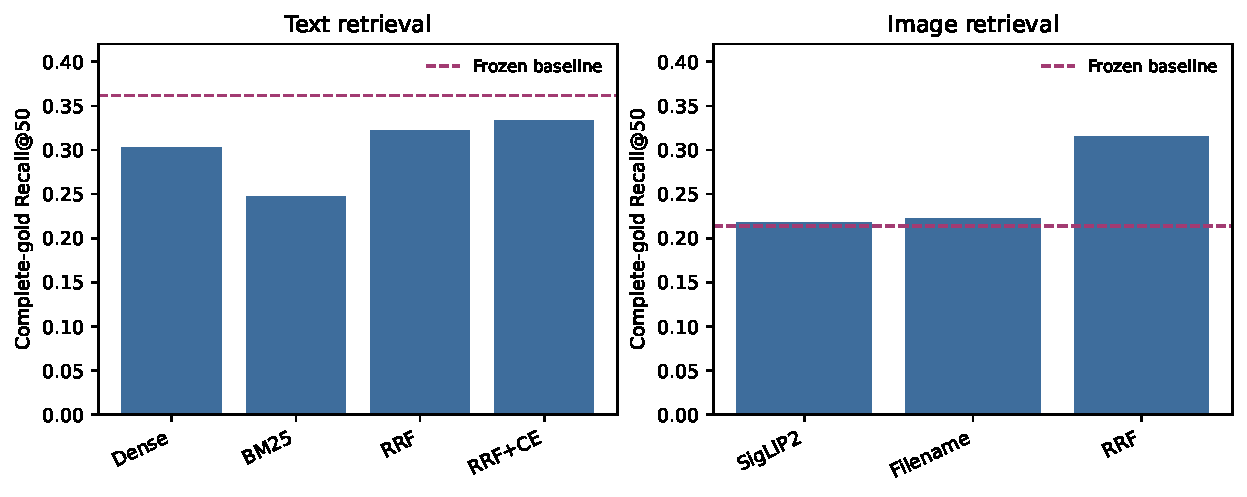
\includegraphics[width=0.92\textwidth]{../research/q1_phase2/figures/retrieval_matrix.pdf}
\caption{Complete-gold Recall@50 for declared text and image retrieval variants. Dashed lines show frozen Phase-1 baselines.}
\label{fig:retrieval}
\end{figure*}

\begin{table}[t]
\centering
\caption{Full retrieval matrix.}
\label{tab:retrieval}
\small
\begin{tabular}{llrr}
\toprule
Modality & Variant & Recall@50 & MAP@100 \\
\midrule
Text & Dense sentence & 0.3028 & 0.1728 \\
Text & BM25 sentence & 0.2478 & 0.1349 \\
Text & Dense--BM25 RRF & 0.3224 & 0.1744 \\
Text & RRF + cross-encoder & 0.3338 & 0.1282 \\
Image & SigLIP2 & 0.2183 & 0.0916 \\
Image & Filename BGE-M3 & 0.2227 & 0.1154 \\
Image & SigLIP2--filename RRF & 0.3149 & 0.1414 \\
\bottomrule
\end{tabular}

\end{table}

\subsection{Scorer and Calibration Gate}

The selected scorer improves model-selection average precision over the shared logistic control in every seed. Seed 13 selects modality-specific logistic scoring; the other four select the cross-encoder-augmented family. Modality temperature scaling improves or preserves Brier score in every seed. Validation Brier decreases from 0.15774--0.16728 raw to 0.15184--0.16295 calibrated. The scorer gate passes, showing that the negative selector result is not caused by retaining the original shared scorer unchanged.

\subsection{Matched Selector Matrix}

Table~\ref{tab:selector} gives five-seed validation means. Fixed top-5 reaches F1 0.16435. Calibrated thresholding is strongest at 0.17863 and improves on fixed by 0.01429, with 95\% CI $[0.01048,0.01814]$. The learned count head over-selects 32.83 items and performs worst.

Original CEFES selects 26.81 items and obtains 0.12227 F1. Size penalties reduce the mean set to 14.89 and improve F1 to 0.14718. \method{} further reduces repeated-source output to 14.73 items but obtains 0.14698 F1. Its mean selected/gold ratio is 1.1809, so the set-size safety condition passes. It nevertheless trails fixed by 0.01737; every seed effect is negative and the aligned CI is $[-0.02264,-0.01222]$.

\begin{table}[t]
\centering
\caption{Five-seed mean complete-gold selector results.}
\label{tab:selector}
\small
\resizebox{\columnwidth}{!}{\begin{tabular}{lrrrr}
\toprule
Method & Precision & Recall & F1 & Selected \\
\midrule
Fixed top-5 & 0.2460 & 0.1718 & 0.1643 & 5.00 \\
Calibrated threshold & 0.2816 & 0.1794 & 0.1786 & 5.53 \\
Learned count & 0.0907 & 0.2818 & 0.1087 & 32.83 \\
CEFES & 0.1002 & 0.2792 & 0.1223 & 26.81 \\
Size-penalized CEFES & 0.1435 & 0.2433 & 0.1472 & 14.89 \\
RC-CEFES & 0.1438 & 0.2421 & 0.1470 & 14.73 \\
\bottomrule
\end{tabular}
}
\end{table}

\begin{figure}[t]
\centering
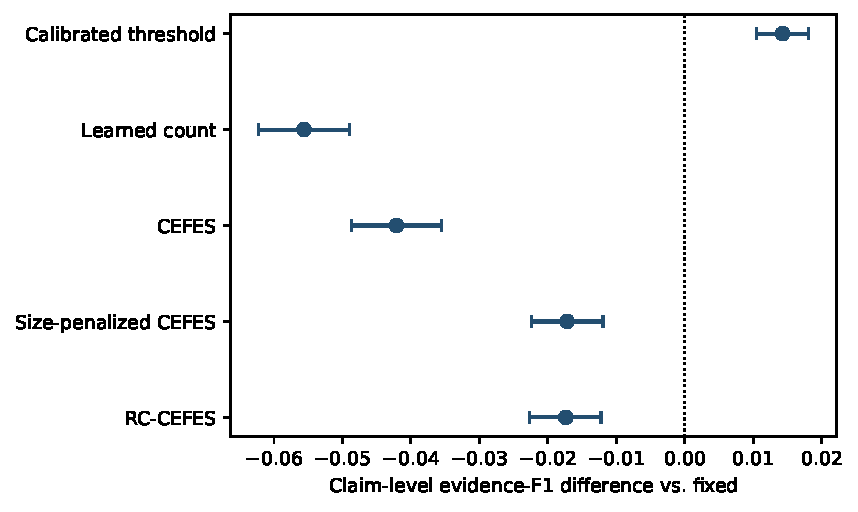
\includegraphics[width=\columnwidth]{../research/q1_phase2/figures/selector_effects.pdf}
\caption{Seed-aligned evidence-F1 effects against fixed top-5. All Holm-adjusted $p$ values are 0.0010.}
\label{fig:selector-effects}
\end{figure}

\begin{table}[t]
\centering
\caption{Seed-aligned selector effects against fixed.}
\label{tab:selector-effects}
\small
\resizebox{\columnwidth}{!}{\begin{tabular}{lrrrr}
\toprule
Method vs. fixed & Mean & 95\% lower & 95\% upper & Holm $p$ \\
\midrule
Calibrated threshold & +0.0143 & +0.0105 & +0.0181 & 0.0010 \\
Learned count & -0.0556 & -0.0623 & -0.0490 & 0.0010 \\
CEFES & -0.0421 & -0.0486 & -0.0355 & 0.0010 \\
Size-penalized CEFES & -0.0172 & -0.0224 & -0.0119 & 0.0010 \\
RC-CEFES & -0.0174 & -0.0226 & -0.0122 & 0.0010 \\
\bottomrule
\end{tabular}
}
\end{table}

\subsection{Shared-Verifier Safeguard}

The mean \method{}--fixed verifier change is $+0.00435$ macro-F1. The aligned interval, $[-0.01126,0.02005]$, crosses zero and its lower bound is below the $-0.01$ margin. The non-inferiority safeguard therefore fails, even though the point estimate is positive. Calibrated thresholding has the highest verifier macro-F1 in every seed.

\begin{figure}[t]
\centering
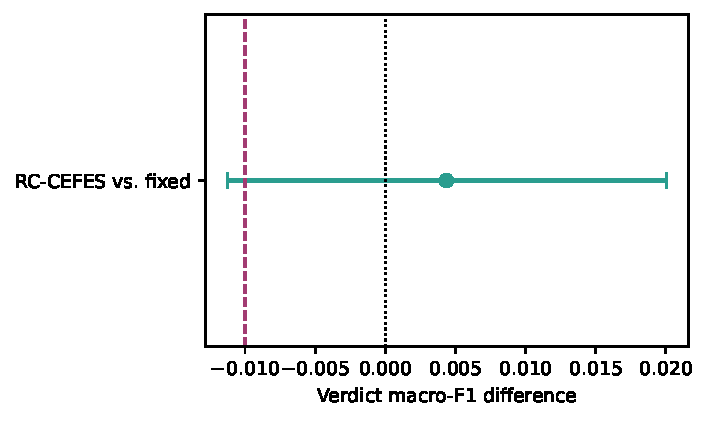
\includegraphics[width=\columnwidth]{../research/q1_phase2/figures/verifier_noninferiority.pdf}
\caption{Shared-verifier effect. The dashed line is the $-0.01$ non-inferiority margin.}
\label{fig:verifier}
\end{figure}

\subsection{Controlled Robustness Diagnostics}

The post-outcome diagnostic protocol perturbs frozen packets without refitting. Figure~\ref{fig:robustness} shows that \method{} remains below fixed for width 20/40, text-only or image-only packets, removal of retrievable gold, and both rank-preserving temperature shifts. At width 10 its interval reaches zero. Duplicating the top three items also yields an interval containing zero, consistent with the redundancy penalty becoming useful.

Promoting five known non-gold candidates to the highest scores produces a large \method{} advantage ($+0.13736$). This is not evidence of ordinary superiority: the intervention deliberately fills fixed top-5 with distractors, while the larger adaptive set can still recover evidence below them. It locates a boundary where a variable set is robust to catastrophic early ranking error.

\begin{figure*}[t]
\centering
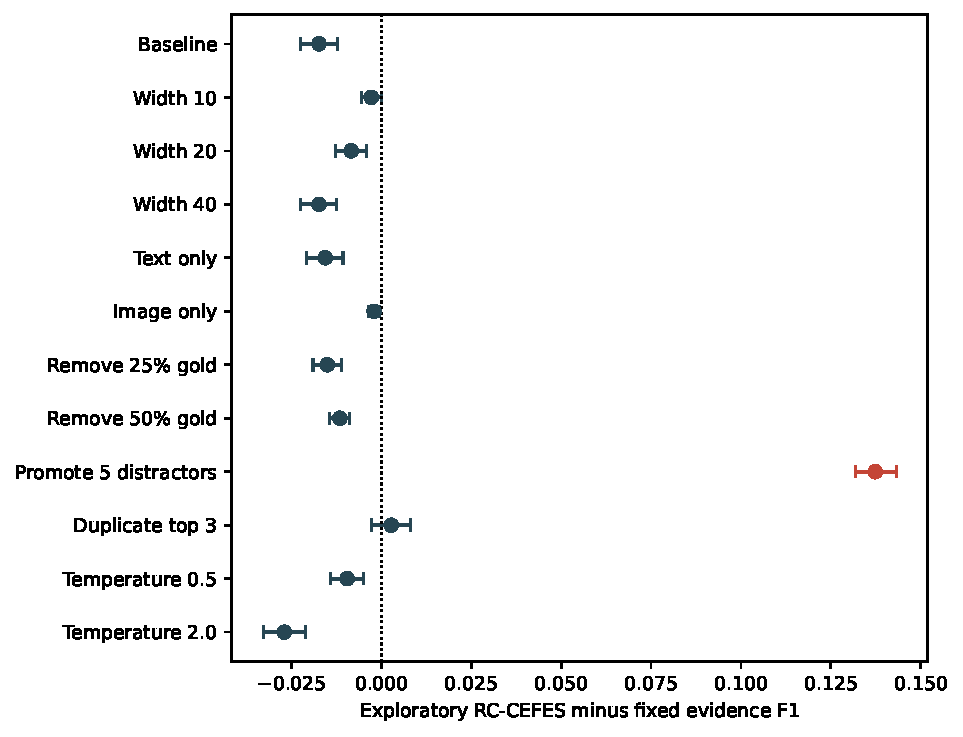
\includegraphics[width=0.82\textwidth]{../research/q1_phase2/figures/robustness_effects.pdf}
\caption{Exploratory five-seed effects under frozen packet perturbations. The highlighted condition deliberately promotes known distractors and has no confirmatory status.}
\label{fig:robustness}
\end{figure*}

\subsection{Reproduction, External Gate, and Final Decision}

A clean run rebuilds retrieval rankings, candidate features, five-seed scorer/selector records, verifier checkpoints, and predictions in a separate namespace. Twenty-seven core artifacts match byte-for-byte. The two label-blind prejoin manifests match after normalizing their expected output-path strings. All six independent audits pass.

AVerImaTeC and MMCV pass licensing/relevance screening but not unchanged-protocol compatibility. AVerImaTeC has no usable released blind test and represents evidence as QA-supported web sources. MMCV adds table evidence, lacks an official fitting/test split, and reports an open-book condition with gold evidence. No external outcome is claimed.

Table~\ref{tab:gate} gives the final conjunctive decision. Text retrieval, selector superiority, and verifier non-inferiority fail. The formal test remains sealed.

\begin{table}[t]
\centering
\caption{Final development gate. Every condition is required.}
\label{tab:gate}
\small
\begin{tabular}{p{0.76\columnwidth}c}
\toprule
Condition & Status \\
\midrule
Text Recall@50 gain at least +0.10 & \textbf{Fail} \\
Image Recall@50 gain at least +0.10 & Pass \\
Selected scorer improves MAP in every seed & Pass \\
Calibrated Brier score is non-worse in every seed & Pass \\
Mean RC-CEFES evidence-F1 gain at least +0.015 & \textbf{Fail} \\
RC-CEFES evidence effect positive in every seed & \textbf{Fail} \\
Seed-aligned evidence interval lower bound above zero & \textbf{Fail} \\
Mean selected/gold evidence ratio no more than 2 & Pass \\
Verifier interval lower bound above -0.01 & \textbf{Fail} \\
Clean end-to-end reproduction & Pass \\
\bottomrule
\end{tabular}

\end{table}

\section{Discussion}

\subsection{What Improved}

The new system does not merely repeat the frozen failure. Image RRF adds about ten Recall@50 points, modality-aware scoring consistently improves ranking, calibration improves Brier score, and precision penalties cut CEFES output by roughly 45\% while raising its F1 by 0.02471. These are meaningful component gains. They show that the original failure was partly addressable without increasing model access for one selector.

\subsection{Why the Main Conclusion Remains Negative}

The improvements do not compose into superiority. Text coverage remains below the frozen baseline and the cross-encoder trades deeper recall for much worse early ranking. Expected-F1 decoding is sensitive to the high membership probabilities assigned to distractors and to dependence among same-source items. Size penalties correct extreme over-selection, but the best precision--recall point is still a global calibrated threshold. This also demonstrates why a method should be compared with both a strong fixed budget and a simple adaptive control.

The verifier reinforces the distinction between evidence and verdict endpoints. Its point effect is favorable, but uncertainty is too wide for the declared non-inferiority claim. More context can help a classifier even when it is not faithful to the released evidence set; the two outcomes should not be substituted.

\subsection{When Adaptivity Helps}

The controlled interventions give a narrow answer. Reducing packet width or retaining only images makes fixed and adaptive selection more similar because little useful depth remains. Duplicate pollution moves \method{} toward parity because its source penalty discourages redundant output. Deliberate top-rank distractor promotion reverses the result because fixed top-5 has no way to look below five corrupted items, whereas an adaptive set can expand. This supports a conditional claim: variable-size selection can hedge against severe early ranking corruption, but the evaluated scorer cannot reliably recognize that condition in ordinary MOCHEG retrieval.

\subsection{Implications for Evaluation}

Candidate construction is part of the scientific claim. Judgment-packet, full-corpus, and perturbed-packet results answer different questions and should not be pooled. Complete-gold scoring, raw ranking preservation before label joins, strong fixed/threshold controls, and chronological gates make those distinctions auditable. A negative upstream gate should narrow the manuscript claim rather than trigger unconstrained decoder search.

\section{Limitations and Ethical Considerations}

This is a single-benchmark development study, not formal-test confirmation. MOCHEG development outcomes were already inspected in earlier work, so the expanded validation check is reused development evidence rather than statistically fresh confirmation. The official test remains sealed. No current second benchmark supports an unchanged replication; MMCV would require a table modality and a newly defined split, while AVerImaTeC would require a new evidence-identity and open-web corpus protocol.

The image system uses filename text but no OCR or generated caption, because those sources were outside the frozen trial budget. Text reranking is expensive (about 19 minutes for the full reranker pass on an RTX 4090) and degrades early precision. The membership models are low-capacity logistic controls rather than fine-tuned multimodal cross-encoders. The expected-F1 decoder assumes conditional independence, although evidence from one article or duplicate group is correlated. Source metadata are insufficient for a source-cluster bootstrap, so claims are the resampling unit.

The 2,189 claims without a released non-empty complete-gold mapping are excluded transparently. This may limit population coverage, but treating them as true empty evidence sets would reward empty predictions and conflate release mapping with task semantics. Controlled robustness is explicitly post-outcome and exploratory. In particular, the positive distractor-promotion result is an artificial stress test and cannot support a deployment claim.

Automated fact-checking may misrepresent people, sources, or events when retrieval is incomplete. The system should support human evidence review, not autonomously adjudicate truth. Public data and model artifacts are used under their research licenses; immutable identifiers and hashes are retained, while credentials and private information are not distributed. Negative results and failed gates are preserved to reduce selective reporting.

\section{Conclusion}

We evaluated adaptive multimodal evidence selection as a retrieval-conditioned pipeline rather than an isolated decoder. Hybrid image retrieval, modality-aware scoring, calibration, and size penalties all improve their intended components. \method{} corrects much of original CEFES's over-selection, but it does not beat fixed top-5 and is clearly weaker than calibrated thresholding on complete-gold evidence F1. Its shared-verifier interval also misses the declared non-inferiority margin.

The result is robust across five seeds, Holm-adjusted paired analysis, independent audits, and an exact clean reproduction. Controlled perturbations clarify the boundary: adaptivity becomes advantageous under deliberate early-rank poisoning, not under ordinary retrieved packets. Because the conjunctive gate fails and no unchanged external benchmark qualifies, the official test remains sealed. The defensible contribution is the framework and the evidence about when selector conclusions change, not a claim that \method{} is superior.


\appendices
\section{Artifact and Failure Record}

The embedding cache contains 13,159 claim vectors, 378,864 sentence vectors, 90,270 filename vectors, and 90,270 image vectors. It required 1,892.27 seconds. The outcome-bearing retrieval pass required 1,155.93 seconds and produced 789,540 candidate rows. Five-seed selector and verifier runs required 153.22 and 254.29 seconds, respectively, excluding the clean rerun.

Two implementation defects were found before finalization and retained in the experiment ledger. The first selector launch included claims absent from the non-empty complete-gold map and failed before writing scientific results. The repair filters by split-qualified complete-gold keys and is covered by a regression test. The first verifier summary reported only per-seed intervals; saved predictions were unchanged while the protocol-required claim-aligned aggregate was added and tested. The final suite contains 115 passing tests.

The complete records are stored under \texttt{experiments/outputs/q1\_phase2/}. Compact reporting artifacts, the protocol, final gate, reproduction manifest, robustness protocol, external access audit, and append-only ledger are stored under \texttt{research/q1\_phase2/}. The frozen Phase-1 manuscript and outputs are not overwritten.


\IEEEtriggeratref{4}
\bibliographystyle{IEEEtran}
\bibliography{references}
\end{document}
